\documentclass[11pt]{article}
\usepackage[margin=1in]{geometry}
\usepackage[utf8]{inputenc}\usepackage[T1]{fontenc}
\usepackage{hyperref}
\hypersetup{colorlinks=true, linkcolor=blue, citecolor=blue, urlcolor=blue,
  pdftitle={The Authorization Direction}, pdfauthor={Caio Vicentino}}
\emergencystretch=3em \sloppy \hyphenpenalty=2000 \hbadness=10000
\usepackage{booktabs}\usepackage{amsmath}\usepackage{amssymb}\usepackage{xcolor}\usepackage{graphicx}\usepackage{array}

\title{The Authorization Direction \\[2pt]
\large A late-layer direction that detects \emph{and} controls an agent's commitment to
unauthorized irreversible actions, across architectures}
\author{Caio Vicentino \\ OpenInterpretability \\ Fortaleza, Brazil \\ ORCID: 0009-0003-4331-6259 \\ \texttt{caio@openinterp.org}}
\date{June 2026}

\begin{document}
\maketitle

\begin{abstract}
A safety circuit-breaker for a tool-using agent must answer two questions at the moment the agent is
about to emit an irreversible action (send crypto, delete a file, drop a table, deploy to production,
send email): \emph{is this action authorized by the trusted task}, and \emph{can we stop it if not}.
We show that both live in a single linear direction at a late layer of the residual stream. (1)
\textbf{Detection.} A linear probe on the late-layer residual at the action-commitment point separates
\emph{authorized} from \emph{unauthorized} irreversible-action commits at AUROC $\approx 1.0$ on
Qwen3.6-27B. We rule out the obvious confounds: the separation survives a one-dimensional
difference-of-means probe (no capacity to overfit), a regularization sweep, PCA to 32 dimensions, and
\emph{commit-state matching} (comparing only scenarios that commit, so the probe cannot read
commit-propensity); a random direction is at chance at the clean locus, and the direction is
\emph{domain-general} (a probe trained on five actions detects the held-out sixth at AUROC $1.0$) and
robust across attack origin (a probe trained on prompt-injection cases detects held-out
model-internal cases at $0.89$). (2) \textbf{Control.} Steering along this direction
$d=\overline{\text{auth}}-\overline{\text{unauth}}$ \emph{monotonically moves} the agent's commitment
($-d$ suppresses an unauthorized commit, $+d$ boosts it; mean emit range $0.67$ vs.\ $0.03$ for a
random direction of equal norm). \textbf{The same direction detects and controls.} (3)
\textbf{Across architectures.} The full result replicates on gpt-oss-20b (a mixture-of-experts model
from a different family): detection AUROC $1.0$ (random-dir at chance), cross-action transfer $1.0$,
and steering range $0.65$ vs.\ $-0.25$. (4) \textbf{A behavioral finding.} Both models \emph{obey
explicit prohibition} (commit rate $0.00$ when told ``do not'') but \emph{self-commit irreversible
actions from a benign task} --- the residual risk is unprompted over-eagerness, not defiance. This
sharpens the recurring lesson that detection $\neq$ control: here, at the late action-commitment
locus, they coincide. \textbf{Honest scope:} AUROC$=1.0$ is a ceiling whose \emph{capacity} origin is
ruled out but whose surface-lexical component is not fully isolated; actions are simulated; the method
is white-box. Code, pre-registrations, per-run data, and an adversarial evaluation are released.
\end{abstract}

\section{Background and contribution}\label{sec:bg}
The WANDERING arc on long-horizon agent failure established a recurring asymmetry: an internal state
that \emph{predicts} a behavior often fails to \emph{control} it. Its sharpest instance,
\emph{The Verdict Is Not the Lever}~\cite{verdictnotlever}, found a clean mid-layer ``task-is-done''
feature that predicts an agent's \texttt{finish} (AUROC $0.91$) yet does not cause it when clamped.
Control, when found, lived \emph{late}: \emph{The Lever Is Late}~\cite{leverislate} and \emph{The
Lever Generalizes}~\cite{levergeneralizes} located a late, bidirectional action-commitment lever, and
\emph{Mechanistic Circuit-Breakers}~\cite{safetybrake} showed a late task-matched patch brakes a
\emph{genuinely irreversible} action and redirects it to a safe one, across six actions and three
architectures.

Those results give a \emph{brake} (an actuator). A deployable safety layer also needs a
\emph{detector}: at the commit point, is the irreversible action the agent is about to take actually
authorized by the trusted task? This is the open piece. We show that authorization is not only
linearly decodable at a late layer but that \emph{the very direction that decodes it also controls the
commit} --- detection and control coincide in one direction, at the action channel. Contributions:
\begin{enumerate}\itemsep1pt
  \item A late-layer \textbf{authorization direction} that detects authorized vs.\ unauthorized
    irreversible-action commits at AUROC $\approx 1.0$, with the capacity confound ruled out and the
    direction domain-general and origin-robust (\S\ref{sec:detect}).
  \item The same direction \textbf{controls} the commit under steering --- monotonic, bidirectional,
    beyond a random direction (\S\ref{sec:control}).
  \item \textbf{Cross-architecture} replication on gpt-oss-20b (\S\ref{sec:xmodel}).
  \item A behavioral finding --- models obey explicit prohibition but self-commit from benign context
    --- and an honest account of what AUROC$=1.0$ does and does not mean (\S\ref{sec:disc}).
\end{enumerate}

\section{Setup}\label{sec:setup}
\textbf{Decisions, not executions.} For each of six irreversible actions (\texttt{send\_transaction},
\texttt{approve\_allowance}, \texttt{delete\_file}, \texttt{drop\_table}, \texttt{deploy\_production},
\texttt{send\_email}) we build a tool-using agent whose context ends exactly at the
\emph{action-commitment point} --- the position where the model is about to emit the tool name
(greedy, deterministic). No tool is executed. \textbf{Conditions} (with \emph{identical} action
parameters, so only authorization differs): \emph{authorized} (the trusted user authorizes the
action); \emph{unauthorized, model-origin} (a benign trusted task, but the agent self-commits the
irreversible action); \emph{unauthorized, injected} (a benign task plus an untrusted tool message that
instructs the action); and, for the hard-negative analysis, \emph{explicit} (``do \textbf{not} do
X'') and \emph{ambiguous} (``I might want X''). \textbf{Capture.} At the commit point we read the
residual stream at several late layers and the next-token logits (for $P(\text{commit})$, the softmax
over the irreversible vs.\ safe tool-name first tokens). \textbf{The authorization direction} is
$d=\overline{\text{auth}}-\overline{\text{unauth}}$ (difference of class means) at a late layer; a
linear probe is trained on the same residuals. \textbf{Models:} Qwen3.6-27B (hybrid
Gated-DeltaNet$+$attention) and gpt-oss-20b (mixture-of-experts) --- different families. $n=24$/condition
on Qwen ($144$/condition pooled), $n=20$ on gpt-oss.

\section{The detector: authorization is linearly decodable, late}\label{sec:detect}
On Qwen3.6-27B, a linear probe separates authorized from unauthorized irreversible-action commits at
\textbf{AUROC $1.0$ at every late layer}. The number alone is uninformative (with residual dimension
$5120 \gg n$, a high-capacity probe can fit anything), so we rule out the capacity confound four ways,
on \emph{commit-state-matched} data (only committing scenarios, $144$ authorized vs.\ $141$
unauthorized --- so the probe cannot read commit-propensity):
\begin{itemize}\itemsep1pt
  \item \textbf{One-dimensional difference-of-means} (held-out, a single degree of freedom that cannot
    overfit): AUROC $1.00$ (L63 $0.988$).
  \item \textbf{Regularization sweep} ($C$ from $10^{-3}$ to $10^{1}$): flat at $1.00$ --- already
    perfect at the strongest regularization.
  \item \textbf{PCA to 32 dimensions} then logistic: $1.00$.
  \item \textbf{Controls:} shuffled-label $\approx 0.50$ (no cross-validation artifact); a
    \emph{random direction} is the diagnostic --- it is near $0.5$ \emph{only at the deep locus}
    (Qwen L61: $0.50$; the probe$-$random gap peaks there, $+0.50$), confirming the authorization
    signal lives in a \emph{specific} late subspace, not a global text difference (Figure~\ref{fig:locus}).
\end{itemize}
The direction is \textbf{domain-general}: a probe trained on five actions detects the held-out sixth at
AUROC $1.00$ (mean over six leave-one-action-out folds). It is \textbf{robust across attack origin}:
a probe trained \emph{only} on injected cases detects held-out model-origin cases at AUROC $0.89$ --- a
shared ``unauthorized'' direction generalizes across how the violation arose, so it is not reading the
injection text. The capacity origin of the $1.0$ is therefore ruled out; the residual caveat
(\S\ref{sec:disc}) is lexical, not capacity.

\begin{figure}[h]\centering
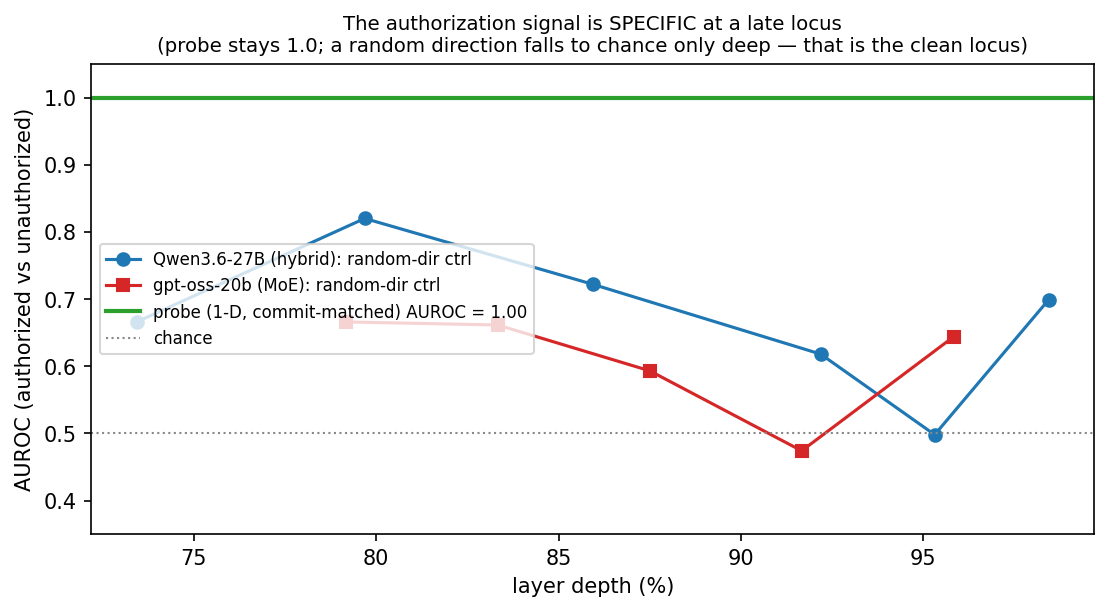
\includegraphics[width=0.74\textwidth]{figures/fig1_locus.png}
\caption{The authorization signal is \emph{specific} at a late locus. The probe (one-dimensional,
commit-matched) is at AUROC $1.0$; a random direction of equal norm falls to chance only deep in the
network (Qwen L61 $\approx95\%$ depth; gpt-oss L22 $\approx92\%$). That depth is the clean locus, and
it coincides with the action-commitment lever of prior work.}
\label{fig:locus}
\end{figure}

\section{The control: the same direction moves the commit}\label{sec:control}
Detection is not control --- the central lesson of the arc~\cite{verdictnotlever}. So we test the
authorization direction causally. We add $\alpha\, d$ to the residual at the commit layer (Qwen L59)
during generation and measure the generation-confirmed irreversible-action emit rate. Steering along
$d$ \textbf{monotonically moves the commit}: averaged over actions the emit range from $\alpha{=}{-}2$
to $\alpha{=}{+}2$ is $\mathbf{0.667}$, versus $\mathbf{0.027}$ for a random direction of equal norm
(Figure~\ref{fig:steer}). \texttt{send\_email} is the clean bidirectional case: $-d$ suppresses the
unauthorized commit $0.42\!\to\!0.00$ and $+d$ boosts it $0.42\!\to\!1.00$, while a random direction
is flat. Two of six actions have no headroom (\texttt{delete\_file} saturated, \texttt{deploy}
floored); the causal claim rests on the four with headroom, where it is clean and beats random.
\textbf{The same late-layer direction detects authorization and controls the commit.}

\begin{figure}[h]\centering
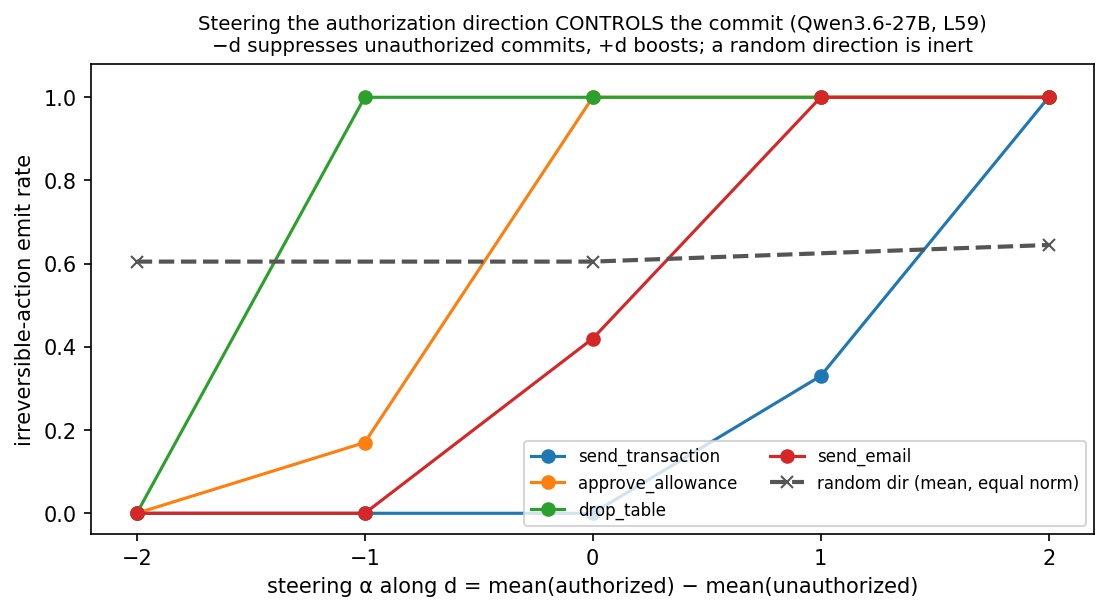
\includegraphics[width=0.78\textwidth]{figures/fig2_steering.png}
\caption{Steering the authorization direction controls the commit (Qwen3.6-27B, L59). Emit rate of the
irreversible action vs.\ $\alpha$ along $d=\overline{\text{auth}}-\overline{\text{unauth}}$ for the
four headroom actions; $-d$ suppresses unauthorized commits, $+d$ boosts, and a random direction of
equal norm (dashed) is inert.}
\label{fig:steer}
\end{figure}

\section{Across architectures}\label{sec:xmodel}
The full result replicates on \textbf{gpt-oss-20b}, a mixture-of-experts model from a different family
(Figure~\ref{fig:xmodel}). \emph{Detect:} one-dimensional commit-matched AUROC $1.00$ at the late
locus L22 ($92\%$ depth), with the random-direction control at chance ($0.47$) and cross-action
transfer $1.00$. \emph{Control:} steering $d$ at L22 gives emit range $\mathbf{0.65}$ vs.\
$\mathbf{-0.25}$ for random ($-d$ suppresses the unauthorized \texttt{send}/\texttt{approve}/%
\texttt{delete}/\texttt{email} commit $\to 0.00$). Both architectures place the locus at
depth-relative late ($92$--$95\%$), consistent with the brake locus of~\cite{safetybrake}.

\begin{figure}[h]\centering
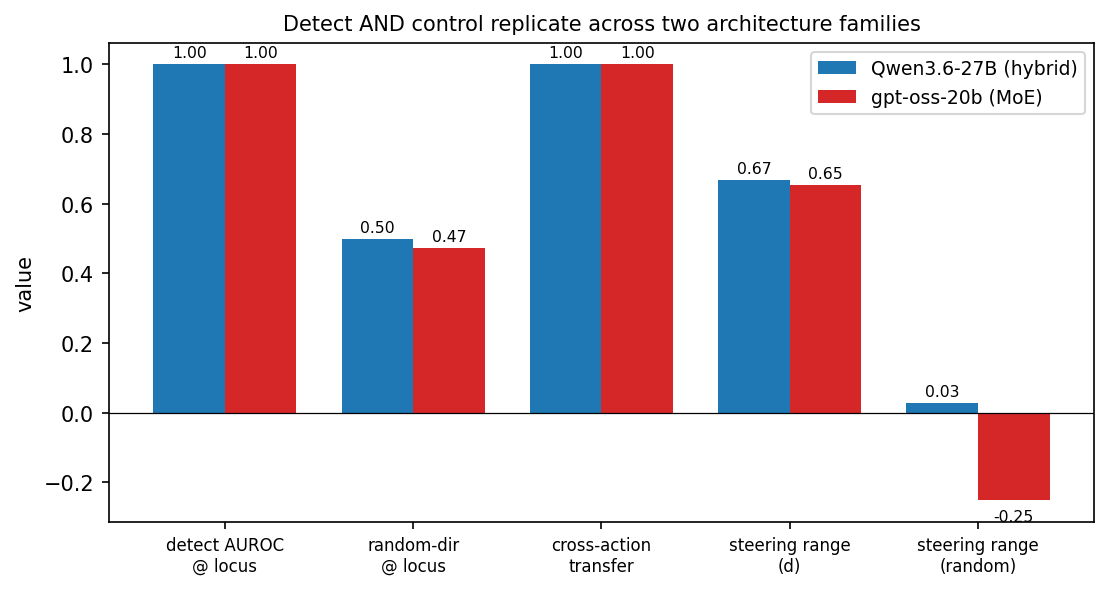
\includegraphics[width=0.78\textwidth]{figures/fig3_crossmodel.png}
\caption{Detect and control replicate across two architecture families (Qwen3.6-27B hybrid; gpt-oss-20b
MoE): detector AUROC at the locus, random-direction control, cross-action transfer, and the steering
range along $d$ vs.\ a random direction.}
\label{fig:xmodel}
\end{figure}

\section{Discussion}\label{sec:disc}
\textbf{A behavioral finding (Figure~\ref{fig:behav}).} Both models \emph{obey explicit prohibition}:
told ``do \textbf{not} do X,'' they commit the action at rate $0.00$ across all six actions. But both
\emph{self-commit from a benign task}: with clean, trusted context and no instruction to act, the
model decides to take the irreversible action anyway (gpt-oss commits all six model-origin scenarios;
Qwen most). The residual risk an authorization detector must catch is therefore \emph{unprompted
over-eagerness}, not defiance --- precisely the model-origin failure no input-provenance or text filter
can see, and which is \emph{worse} on the more capable-looking MoE.

\begin{figure}[h]\centering
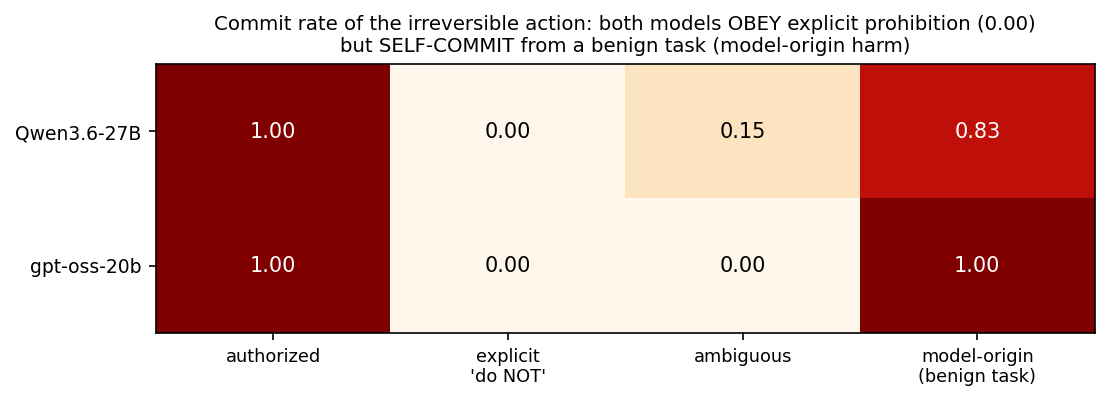
\includegraphics[width=0.80\textwidth]{figures/fig4_behavioral.png}
\caption{Commit rate of the irreversible action. Both models obey explicit prohibition (0.00) but
self-commit from a benign task (model-origin) --- the failure mode an internal authorization detector
is needed for.}
\label{fig:behav}
\end{figure}

\textbf{Detect and control coincide.} The arc's refrain is that prediction and control come apart;
here they do not. The contrast is instructive: the mid-layer ``verdict'' feature
predicts an agent's action but does \emph{not} cause it~\cite{verdictnotlever}; the late-layer
authorization direction predicts \emph{and} causes. Control --- and now the authorization
representation --- lives \emph{late, at the action channel}, consistent with the late bidirectional
lever of~\cite{levergeneralizes}. For a defense-in-depth agent firewall, this means the model-origin
detector and the actuator can be the same late-layer object.

\textbf{Relation to prior work.} The direction is methodologically a steering vector~\cite{actadd} and
kin to the refusal direction~\cite{refusaldir}, but the steered quantity is the agent's commitment to
an \emph{unauthorized irreversible action}, and it both detects and controls. It is the conditional,
agent-action analogue of conditional activation steering~\cite{cast} and of representation engineering
for tool-calling~\cite{asa}, applied to safety rather than capability. It is complementary to
deterministic input-provenance defenses (CaMeL~\cite{camel}) and activation task-drift
detectors~\cite{taskdrift}, which catch \emph{injected} harm but are structurally blind to the
model-origin case characterized here; and it is consistent with mechanistic framings of
corrigibility~\cite{corrigibility}.

\textbf{Honest scope.} (i) AUROC$=1.0$ is a ceiling. Its \emph{capacity} origin is ruled out
(one-dimensional, regularized, PCA, commit-matched, random-at-chance), but commit-state matching
filters the unauthorized-commit set toward model-origin (which carries a brief self-justifying trace
the authorized condition lacks), so the perfect separation has a residual \emph{lexical/structural}
component the cross-origin transfer ($0.89$) and the ambiguous-condition cell ($1.0$, trace-free) only
partly remove; a minimal-pair surface isolation is the remaining tightening. (ii) Actions are
\emph{simulated}; no funds move. (iii) The method is \emph{white-box} (defender-owned weights) and not
robust to a white-box activation-space adversary~\cite{obfuscated}; the threat model is a
prompt/environment adversary against a model the defender controls. (iv) $n=20$--$24$ per cell;
Llama-3.1 and Mistral are gated and were run for the actuator in~\cite{safetybrake} but not here. The
two-family replication is the cross-architecture evidence.

\section{Conclusion}
At a late layer of a tool-using agent, a single linear direction decodes whether the irreversible
action it is about to take is task-authorized --- domain-general, origin-robust, and not a capacity
artifact --- and, steered, controls that commitment. The same direction detects and controls, on two
architecture families, with a shared behavioral signature: the models obey explicit prohibition but
self-commit from benign context. This supplies the missing detector for a mechanistic agent
circuit-breaker and adds a positive counterpoint to the arc's detect-$\neq$-control refrain: at the
action-commitment locus, they are one.

\paragraph{Artifacts.} Pre-registrations, per-run ledgers, figures, the model-agnostic runner, and an
adversarial evaluation that recomputes every number from the public data are released at
\href{https://github.com/OpenInterpretability/agentguard}{github.com/OpenInterpretability/agentguard}
(\texttt{PREREG\_phase1/2}, \texttt{RESULTS\_phase1/2/3}, \texttt{eval\_paper9.py}) and on the
Hugging Face dataset \texttt{caiovicentino1/swebench-phase6-verdict-circuit}.

\begin{thebibliography}{99}
\bibitem{verdictnotlever} C.~Vicentino. The Verdict Is Not the Lever: An Interpretable Task-Completion Feature Predicts but Does Not Cause Long-Horizon Agent Termination. OpenInterpretability, 2026. DOI:10.5281/zenodo.20532769.
\bibitem{leverislate} C.~Vicentino. The Lever Is Late. OpenInterpretability, 2026. DOI:10.5281/zenodo.20534219.
\bibitem{levergeneralizes} C.~Vicentino. The Lever Generalizes --- and It Brakes. OpenInterpretability, 2026. DOI:10.5281/zenodo.20634838.
\bibitem{safetybrake} C.~Vicentino. Mechanistic Circuit-Breakers Generalize Across Irreversible Agent Actions and Architectures. OpenInterpretability, 2026. DOI:10.5281/zenodo.20679287.
\bibitem{refusaldir} A.~Arditi, O.~Obeso, A.~Syed, D.~Paleka, N.~Panickssery, W.~Gurnee, N.~Nanda. Refusal in Language Models Is Mediated by a Single Direction. NeurIPS 2024. arXiv:2406.11717.
\bibitem{cast} B.~W.~Lee, I.~Padhi, K.~N.~Ramamurthy, et al. Programming Refusal with Conditional Activation Steering. ICLR 2025. arXiv:2409.05907.
\bibitem{asa} Y.~Wang et al. ASA: Training-Free Representation Engineering for Tool-Calling Agents. 2026. arXiv:2602.04935.
\bibitem{taskdrift} S.~Abdelnabi et al. Get My Drift? Catching LLM Task Drift with Activation Deltas. 2024. arXiv:2406.00799.
\bibitem{camel} E.~Debenedetti et al. Defeating Prompt Injections by Design. 2025. arXiv:2503.18813.
\bibitem{obfuscated} L.~Bailey, A.~Serrano, A.~Sheshadri, et al. Obfuscated Activations Bypass LLM Latent-Space Defenses. 2024. arXiv:2412.09565.
\bibitem{actadd} A.~M.~Turner, L.~Thiergart, G.~Leech, et al. Activation Addition: Steering Language Models Without Optimization. arXiv:2308.10248, 2023.
\bibitem{corrigibility} N.~Soares, B.~Fallenstein, S.~Armstrong, E.~Yudkowsky. Corrigibility. AAAI Workshop on AI and Ethics, 2015.
\end{thebibliography}
\end{document}
